\documentclass[a4paper, pdftex,final, oneside, 2.8headlines]{scrartcl}

\setcounter{secnumdepth}{4}
\setcounter{tocdepth}{4}

\newcommand{\doctitle}{Hardwareplattformen und Systemsoftware 
f�r drahtlose vermaschte Kommunikationsnetze} % Dokumententitel
\newcommand{\version}{1.1.1} %Versionsnummer


%\usepackage[automark]{scrpage2}  % Kopf-/ Fusszeilen Version 1
%%erfordert in documentclass noch: headsepline, headinclude!
%\pagestyle{scrheadings}

\usepackage[automark]{scrpage2} % Kopf-/ Fusszeilen Version 2
\pagestyle{scrheadings}
\ohead{
\includegraphics[height=1.2cm]{logo}}
\chead{}
\ihead{}

\usepackage{typearea} % Berechnung des Seitenspiegels
\usepackage{listings} % Code-Listings
\usepackage[pdftex]{graphicx}
\graphicspath{{images/}}
\usepackage[ngerman]{babel}
\usepackage[latin1]{inputenc}
\usepackage[T1]{fontenc}
\usepackage{ae,aecompl}
\usepackage[pdftex,hyperref,dvipsnames]{xcolor}
\usepackage{microtype} % optischer Randausgleich
\usepackage{array}
\usepackage{listings}
\usepackage{makecell}
\usepackage{color}

% Anfuehrungszeichen
\usepackage{xspace}
\newcommand{\enquote}[1]{\glqq #1\grqq \xspace}
\newcommand{\mc}[3]{\multicolumn{#1}{#2}{#3}}

% Links und PDF-Spezifika
\pdfcompresslevel=9   % Grafiken komprimieren
\usepackage[pdftex]{hyperref}
\definecolor{darkblue}{rgb}{0,0,.5}
\hypersetup{colorlinks=true, breaklinks=true, linkcolor=darkblue, 
menucolor=darkblue, pagecolor=darkblue, urlcolor=darkblue}
\hypersetup{pdftitle={\doctitle}}
\hypersetup{pdfsubject={Fachstudie "mesh"}}
\hypersetup{pdfauthor={S. Telejnikov, A. Egorenkov}}

\usepackage{float}
\restylefloat{figure}
\restylefloat{table}

\usepackage{hypcap}
\usepackage{thumbpdf}

% Farben:
\definecolor{todoDescription}{rgb}{0.5, 0.0, 0.75} 

%% Befehle f�r ToDos
\newcommand{\todo}[1][TODO]{\textcolor{red}{\textdagger}\marginpar{\tiny{\textbf{
\textcolor{todoDescription}{#1}}}}}

% Absatz Layout
\parindent 0cm
\parskip 2ex

% wlandevice environment
\newenvironment{wlandevice}[1]
{\newpage\paragraph{#1}\label{#1} \begin{description}}
{\end{description}}

\newcommand{\wlanimage}[2]
{
	\begin{figure}[H]
		\centering
		\capstart
		\includegraphics[width=0.5\textwidth]{#1}
		\caption{#2}
	\end{figure}
}

\newcommand{\wlanchipset}[1]
{\item[Chipsatz:] \rule{0mm}{0mm} \begin{itemize} \item #1 \end{itemize}}
\newcommand{\wlanprice}[1]
{\item[Preis:] \rule{0mm}{0mm} \begin{itemize} \item ca. #1 Euro \end{itemize}}

\newenvironment{wlanieeestandard}
{\item[IEEE Standards:] \rule{0mm}{0mm} \begin{itemize}}
{\end{itemize}}

\newenvironment{wlansecurity}
{\item[Sicherheit:] \rule{0mm}{0mm} \begin{itemize}}
{\end{itemize}}

\newenvironment{wlanmode}
{\item[Betriebsart:] \rule{0mm}{0mm} \begin{itemize}}
{\end{itemize}}

\newenvironment{wlandriver}
{\item[Treiber:] \rule{0mm}{0mm} \begin{itemize}}
{\end{itemize}}

\newenvironment{wlanfirmware}
{\item[Firmware:] \rule{0mm}{0mm} \begin{itemize}}
{\end{itemize}}

\newenvironment{wlaninstall}
{\item[Installation:] \rule{0mm}{0mm} \begin{itemize}}
{\end{itemize}}

\newenvironment{wlanextrainfo}
{\item[Weitere Informationen:] \rule{0mm}{0mm} \begin{itemize}}
{\end{itemize}}

\newenvironment{wlanlink}
{\item[Links:] \rule{0mm}{0mm} \begin{itemize}}
{\end{itemize}}

\definecolor{shelllstbgcolor}{gray}{.80}

\lstnewenvironment{shelllst}
{\lstset{language=bash,backgroundcolor=\color{shelllstbgcolor}}}
{}

\begin{document}


%---------------------------------------------------------------------&
% Titelseite

\begin{titlepage}

\begin{figure}[h]
\centering
\hfill
\begin{minipage}{0.2\textwidth}

\includegraphics[width=1.0\textwidth]{images/uni_logo.jpg}
\end{minipage}
\begin{minipage}{0.7\textwidth}
{\Huge\bf Universit\"at Stuttgart}\\[12pt]
{\Large\bf Fakult\"at Informatik, Elektrotechnik\\und Informationstechnik}
\end{minipage}
\end{figure}

\begin{figure}[h]
\centering
\begin{minipage}{0.2\textwidth}

\includegraphics[width=1.0\textwidth]{images/nexus_logo.jpg}
\end{minipage}
\end{figure}

\vspace{30pt}

\begin{center}
Fachstudie Nr. XXXX
\end{center}

\begin{center}
\Large\bf
Hardwareplattformen und Systemsoftware f\"ur drahtlose\\
vermaschte Kommunikationsnetze
\end{center}

\begin{center}
Alexander Egorenkov\\
Sergey Telejnikov\\
Valeri Schneider
\end{center}

\vspace{30pt}

\begin{center}
\begin{tabular}{l@{\hspace{30pt}}l}
\bf Studiengang: & Softwaretechnik\\[5pt]
\bf Pr\"ufer:    & Prof. Dr. Kurt Rothermel\\[5pt]
\bf Betreuer:    & Dipl.-Inf. Lars Geiger\\[5pt]
\bf begonnen am: & November 2007\\[5pt]
\bf beendet am:  & Januar 2008\\[5pt]
\end{tabular}
\end{center}

\vfill

\begin{figure}[h]
\centering
\begin{minipage}{0.2\textwidth}

\includegraphics[width=1.0\textwidth]{images/ipvs_logo.jpg}
\end{minipage}
\begin{minipage}{0.4\textwidth}
\begin{center}
Institut f\"ur Parallele\\
und Verteilte Systeme\\
Abteilung Verteilte Systeme\\
Universit\"atsstra{\ss}e 38\\
D-70569 Stuttgart
\end{center}
\end{minipage}
\begin{minipage}{0.2\textwidth}

\includegraphics[width=1.0\textwidth]{images/vs_logo.jpg}
\end{minipage}
\end{figure}

\end{titlepage}



%\newpage
%\begin{abstract}

	\begin{center}
		\textbf{Abstract}
	\end{center}
	
{\em
	Mesh-Netze (engl. Wireless Mesh Network, WMN) 
	sind drahtlose Ad-Hoc-Netze bestehend aus station"aren 
	Mesh-Routern, die einen Routing-Backbone bilden, 
	und mobilen oder station"aren Mesh-Clients. 
	Die Mesh-Clients kommunizieren uber den Backbone 
	mit anderen Mesh-Clients oder erlangen "uber den 
	Backbone Zugang zum Internet. 
	Mesh-Netze k"onnen dabei auch gr"o"sere Bereiche, 
	beispielsweise ganze St"adte abdecken 
	(entsprechende Stadtnetze werden 
	aktuell z.B. durch Google installiert). 
	
	Ein entsprechendes Mesh-Netz muss f"ur die Forschungszwecke 
	f"ur den Sonderforschungsbereich (SFB) Nexus an der 
	Universit"at Stuttgart eingerichtet werden.
	
	Diese Fachstudie befasst sich mit der Ausarbeitung einer 
	Empfehlung f"ur die Beschaffung entsprechender Ger"ate 
	(Hardwareplattformen und Systemsoftware) f"ur
	den Aufbau eines WMN.
}

%\end{abstract}

%---------------------------------------------------------------------&
\clearpage
\pdfbookmark[1]{Inhaltsverzeichnis}{Inhaltsverzeichnis}
\tableofcontents

%---------------------------------------------------------------------&
%\newpage
\clearpage
\pdfbookmark[1]{Abbildungsverzeichnis}{Abbildungsverzeichnis}
\listoffigures

%---------------------------------------------------------------------&
\clearpage
\setcounter{page}{1}
\section{Einleitung}

In diesem Abschnitt werden einige wichtige Begriffe, die im Laufe des
Dokuments auftauchen werden, kurz erl"autert.

\subsection{Grundlagen von Mesh-Netzen}

\subsubsection{Hintergrund}

Ein drahtloses vermaschtes Netz (engl. Wireless Mesh Network, WMN) besteht
aus einer Menge von Knoten, die "uber drahtlose Kommunikationstechniken
wie beispielsweise IEEE 802.11 (\ref{ieee80211abg}) Nachrichten austauschen. Die
Vemaschung der Knoten erm"oglicht dabei nicht nur den Austausch von
Nachrichten zwischen unmittelbar benachbarten Knoten, sondern auch die
Vermittlung von Nachrichten an entfernte Knoten "uber mehrere Knoten
hinweg. Die Vermittlungsfunktionalit"at wird dabei oft von dedizierten
Vermittlungsknoten (engl. Mesh Router) bereitgestellt, die somit eine
drahtlose Kommunikationsinfrastruktur f"ur die Klienten (engl. Mesh
Client) bilden. Durch den Einsatz vergleichsweise kosteng"unstiger
Hardwarekomponenten und die Vermaschung der Knoten erm"oglichen WMNs die
kosteng"unstige Vernetzung auch gr"o"serer Gebiete. Entsprechende Netze
werden beispielsweise von Community-Projekten wie das Freifunk-Projekt (\ref{other_mesh_projects})
oder Firmen wie Google ((\ref{other_mesh_projects}) bereits heute in der Praxis f"ur den Aufbau gr"o"serer
Netze eingesetzt, um beispielsweise kosteng"unstige Internetzug"ange f"ur
Stadtteile oder ganze St"adte zu realisieren.

WMNs sind auch f"ur den Sonderforschungsbereich (SFB) Nexus an der
Universit"at Stuttgart \cite{nexus} von gro"sem Interesse. Im
Zentrum der Forschungen des SFB stehen Umgebungsmodelle f"ur mobile
kontextbezogene Systeme. Umgebungsmodelle sind digitale Abbilder der
physischen Welt, die von kontextbezogenen Systemen genutzt werden, um
sich selbst"andig an die physische Umgebung des Benutzers anzupassen. Ein
einfaches Beispiel sind ortsbezogene Anwendungen, die beispielsweise
aufgrund der aktuellen geographischen Position eines Ger"ats automatisch
Informationen "uber nahe Restaurants, Sehensw"urdigkeiten, usw. selektieren
k"onnen. Zur Kommunikation, insbesondere mit mobilen Ger"aten, werden dabei
hybride Systeme betrachtet, in denen sowohl eine infrastrukturbasierte
Kommunikation als auch die direkte Ad-hoc-Kommunikation zwischen
mobilen Endsystemen m"oglich ist. Hierbei spielen WMNs als eine spezielle
Auspr"agung eines hybriden Kommunikationssystems eine wesentliche Rolle.


\subsubsection{Ad-Hoc}

Ein Ad-hoc-Netz (lat. ad hoc, sinngem"a"s f"ur diesen Augenblick gemacht)
ist ein drahtloses Rechnernetz, das zwei oder mehr Endger"ate zu einem
vermaschten Netz verbindet. Netze, die sich selbst"andig aufbauen und
konfigurieren, nennt man auch mobile Ad-hoc-Netze (engl. mobile ad hoc
network, MANet) oder Mesh-Netze (engl. mesh, Masche, Netz).

Ad-hoc-Netze verbinden mobile Ger"ate (Netzknoten) wie
Mobiltelefone, Personal Digital Assistants und Notebooks ohne
feste Infrastruktur wie Wireless Access Points. Daten werden von
Netzknoten zu Netzknoten weitergereicht, bis sie ihren Empf"anger
erreicht haben, wodurch sich die Datenlast vorteilhafter verteilt
als in Netzen mit zentraler Anlaufstelle. Knappe Ressourcen
wie Rechenzeit, Energie und Bandbreite fordern eine effektive
Zusammenarbeit der Netzknoten. Spezielle Routingverfahren sorgen
daf"ur, dass sich das Netz best"andig anpasst, wenn sich Knoten
bewegen, hinzukommen oder ausfallen.

\subsubsection{Mesh-Netz}

In einem vermaschten Netz (Mesh-Netz) ist jeder Netzwerkknoten mit einem
oder mehreren anderen verbunden. Die Informationen werden von Knoten
zu Knoten weitergereicht, bis sie das Ziel erreichen. Vermaschte
Netze sind im Regelfall selbstheilend und dadurch sehr zuverl"assig:
Wenn ein Knoten oder eine Verbindung blockiert ist oder ausf"allt, kann
sich das Netz darum herum neu stricken. Die Daten werden umgeleitet und
das Netzwerk ist nach wie vor betriebsf"ahig. 

Vorteile eines vermaschten Funknetzes:
\begin{itemize}
\item Sicherste Variante eines Netzwerkes
\item Bei Ausfall eines Endger"ates ist durch Umleitung die
Datenkommunikation weiterhin m"oglich
\item Sehr leistungsf"ahig
\item Gute Lastverteilung
\item Niedrige Netzwerkkosten
\item Keine zentrale Verwaltung
\end{itemize}

Nachteile eines vermaschten Funknetzes:
\begin{itemize}
\item Vergleichsweise komplexes Routing n"otig
\item Speichern von Routing-Tabellen in jedem Endger"at
\item Jedes Endger"at arbeitet als Router und ist demnach oft aktiv
\item Die Endger"ate sollten m"oglichst eingeschaltet bleiben
\item H"oherer Stromverbrauch im Endger"at
\end{itemize} 

\subsubsection{IEEE 802.11a/b/g}
\label{ieee80211abg}

\textbf{IEEE 802.11} (auch: Wireless LAN, WLAN, WiFi) bezeichnet eine IEEE-Norm
f"ur drahtlose Netzwerkkommunikation. Herausgeber ist das Institute of
Electrical and Electronics Engineers (IEEE).

\textbf{802.11a} spezifiziert eine weitere Variante der physikalischen Schicht,
die im 5-GHz-Band arbeitet und "Ubertragungsraten bis zu 54 MBit/s
ermoglicht. 

\textbf{Vorteile }
\begin{itemize}
	\item weniger genutztes Frequenzband, dadurch h"aufig
	st"orungsfreierer Betrieb m"oglich 
	\item in Deutschland 19 (bei BNetzA-Zulassung) nicht "uberlappende
	Kan"ale 
	\item h"ohere Reichweite, da mit 802.11h bis zu 1000 mW Sendeleistung
	m"oglich 
\end{itemize}

\textbf{Nachteile }
\begin{itemize}
	\item st"arkere Regulierungen in Europa: auf den meisten Kan"alen DFS
	n"otig 
	\item auf einigen Kan"alen kein Betrieb im Freien erlaubt 
	\item falls kein TPC benutzt wird, muss die Sendeleistung reduziert
	werden 
	\item Ad-hoc-Modus wird von den meisten Ger"aten
		nicht unterst"utzt
	\item geringere Verbreitung, daher wenig verf"ugbare Ger"ate
		auf dem Markt und hohe Kosten
\end{itemize}

\textbf{802.11b} ist ebenfalls eine alternative Spezifikation der physikalischen
Schicht, die mit dem bisher genutzten 2,4-GHz-Band auskommt und
"Ubertragungsraten bis zu 11 MBit/s erm"oglicht. 

\textbf{Vorteile}
\begin{itemize}	
	\item gebuhrenfreies freigegebenes ISM-Frequenzband 
	\item hohe Verbreitung und daher geringe Ger"atekosten 
\end{itemize}

\textbf{Nachteile}
\begin{itemize}	
	\item Frequenz muss mit anderen Ger"aten/Funktechniken geteilt werden
	(Bluetooth, Mikrowellenherde, etc.) 
	\item st"orungsfreier Betrieb von nur maximal 3 Netzwerken
	am selben Ort m"oglich, da effektiv nur 3 brauchbare
	(kaum "uberlappende) Kan"ale zur Verf"ugung stehen
	(in Deutschland: 1, 7, 13) 
\end{itemize}

\subsubsection{Ad-Hoc Routing-Protokolle}

Ein Ad-hoc Netzwerk beispielsweise ein Sensornetzwerk besteht aus einer
gro"ser Anzahl von Knoten, die sich typischerweise spontan vernetzen
m"ussen. "Uber Funk k"onnen diese Knoten miteinander kommunizieren. Aber
Knoten kann wegen der Leistungsf"ahigkeit, des Energieverbrauches
und auch der Mobilit"at nicht mit allen anderen Knoten direkt Daten
"ubertragen. Routing Methoden bieten die M"oglichkeit, Kommunikation
zwischen zwei Knoten mit Hilfe der anderen Knoten auszuf"uhren, wenn die
zwei Knoten miteinander nicht direkt kommunizieren k"onnen.

Es gibt mehr als 70 konkurrierende Entw"urfe f�r das Routing der Pakete
durch ein Mobiles Ad-Hoc/Maschennetzwerk. Eine Klassifikation der
Routingprotokolle kann durch Anzahl der Empf"anger getroffen werden:
\begin{itemize}
\item unicast Routing - Ziel der Daten"ubertragung ist ein einzelner Knoten
\item multicast Routing - Ziel sind mehrere Knoten
\item geocast Routing - Ziel sind alle Knoten in einem bestimmten
geografischen Bereich
\item broadcast Forwarding - Ziel sind alle Knoten in der Reichweite
des Senders
\end{itemize}

Eine andere M"oglichkeit der Klassifikation besteht in der Einteilung
der Protokolle hinsichtlich des grunds"atzlichen Ansatzes. Diese Ans"atze
werden im Folgenden vorgestellt.

\textbf{Positionsbasierte Routingverfahren}

Positionsbasierte Routingverfahren nutzen geod"atische Informationen "uber
die genauen Positionen der Knoten. Diese Informationen werden z. B. "uber
GPS-Empf"anger gewonnen. Anhand dieser Ortsinformationen l"asst sich der
k"urzeste oder der beste Pfad zwischen Quell- und Zielknoten bestimmen. Ein
Beispiel f"ur ein positionsbasiertes Routingprotokoll ist LAR.

\textbf{Topologiebasierte Routingverfahren}

Die topologiebasierten Routingverfahren kommen ohne geod"atische
Informationen "uber die Positionen der Knoten des mobilen
Ad-hoc-Netzes aus. Ihnen gen"ugen logische Informationen "uber die
Nachbarschaftsbeziehungen der Knoten, also welche Knoten eine direkte
Verbindung haben oder "uber einen oder mehrere Zwischenknoten (hop)
in Verbindung treten k"onnen. Diese Nachbarknoten k"onnen miteinander
kommunizieren. Die topologischen Informationen werden meistens durch
den Versand so genannter HELLO-Pakete gewonnen. Je nach Zeitpunkt des
Aufbaus der Topologiedatenbasis handelt es sich um proaktives oder
reaktives Routing. Ein Beispiel f"ur ein Protokoll aus dieser Klasse ist
das Neighbourhood Discovery Protocol (NHDP), das Elemente des Optimized
Link State Routing Protocol (OLSR) verwendet.

\textbf{Proaktive Verfahren}

Proaktive Routingverfahren bestimmen die zu verwendenden Pfade zwischen
zwei Knoten bereits, bevor diese f"ur die "Ubertragung von Nutzdaten
ben"otigt werden. Sollen dann Nutzdaten verschickt werden, so muss nicht
auf die Bestimmung des Pfads zum Zielknoten gewartet werden. Nachteilig
ist daf"ur jedoch, dass diese Verfahren auch ohne Verkehr von Nutzdaten
viele Kontrollpakete verschicken, um Pfade zu bestimmen, die wom"oglich
sp"ater nicht ben"otigt werden. Ein Beispiel f"ur ein Protokoll aus dieser
Klasse ist das Optimized Link State Routing Protocol (OLSR).

\textbf{Reaktive Verfahren}

Im Gegensatz zu den proaktiven Verfahren bestimmen reaktive
Routingverfahren f"ur mobile Ad-hoc-Netze die ben"otigten Pfade zwischen
zwei Knoten erst, wenn Nutzdaten "ubertragen werden sollen. Daraus ergibt
sich, dass das erste Datenpaket einer Verbindung erst mit Verz"ogerung
versendet werden kann, da zun"achst auf den Abschluss der Routenbestimmung
gewartet werden muss. Daf"ur werden allerdings auch nur Kontrollpakete
versendet, wenn Nutzdaten verschickt werden und dies zur Routenbestimmung
notwendig ist. Dies schl"agt sich positiv im Energieverbrauch der Knoten
nieder. Das Protokoll Ad hoc On-Demand Distance Vector (AODV) ist ein
Beispiel f"ur ein Protokoll dieser Kategorie.

\textbf{Hybride Verfahren}

Hybride Verfahren kombinieren proaktive und reaktive
Routingverfahren. Dabei soll das Ziel erreicht werden, die
Vorteile der beiden Ans"atze in einem neuen Routingprotokoll
zusammenzufassen. Beispielsweise kann in einem lokal beschr"ankten Bereich
ein proaktives Verfahren eingesetzt werden, w"ahrend f"ur weiter entfernte
Ziele ein reaktives Verfahren eingesetzt wird. Dies vermindert die
Belastung des Netzes durch Kontrollpakete, die bei einem rein proaktiven
Verfahren "uber das gesamte Netz versendet w"urden. Trotzdem stehen f"ur
lokale Ziele sofort Pfade zur Verf"ugung, ohne dass auf deren Bestimmung
wie bei einem rein reaktiven Verfahren gewartet werden m"usste. ZRP ist
ein Routingprotokoll, das diesen Ansatz umsetzt.

\paragraph{OLSR}
\mbox{}
\begin{figure}[H]

\includegraphics{Olsrd_logo.png}
\end{figure}

Optimized Link State Routing, kurz OLSR, ist ein Routingprotokoll
f"ur mobile Ad-hoc-Netze, das eine an die Anforderungen eines mobilen
drahtlosen LANs angepasste Version des Link State Routing darstellt. Es
wurde von der IETF mit dem RFC 3626 standardisiert. Bei diesem
verteilten flexiblen Routingverfahren ist allen Routern die vollst"andige
Netztopologie bekannt, sodass sie von Fall zu Fall den k"urzesten Weg zum
Ziel festlegen k"onnen. Als proaktives Routingprotokoll h"alt es die daf"ur
ben"otigten Informationen jederzeit bereit. Ein in Mesh-Netzwerken
bekannter Vertreter von LSR ist OLSR von olsr.org. Inzwischen existieren
f"ur OLSR spezielle Erweiterungen. Mit der ETX-Erweiterung wird dem
Umstand Rechnung getragen, dass Links asymmetrisch sein k"onnen. Mit
dem Fisheye-Algorithmus ist OLSR auch fur gro"sere Netzwerke brauchbar
geworden, da Routen zu weiter entfernten Knoten weniger h"aufig neu
berechnet werden. Der entscheidende Nachteil ist aber der trotz
Fisheye-Algorithmus noch recht hohe Rechenaufwand von OLSRD, sobald
die Anzahl an Knoten ein gewisses Ma"s ubersteigt.

\paragraph{B.A.T.M.A.N.}
\mbox{}
\begin{figure}[H]
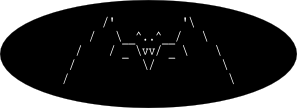
\includegraphics{Batman_logo.png}
\end{figure}

Ausgehend von den Erfahrungen mit Freifunk-OLSR \cite{elektra2007}
begannen die Entwickler
aus der Freifunk-Community im M"arz 2006 in Berlin damit, ein neues
Routingprotokoll f"ur drahtlose Meshnetzwerke zu entwickeln. Alle bisher
bekannten Routingalgorithmen versuchen Routen entweder zu berechnen
(proaktive Verfahren) oder sie dann zu suchen, wenn sie gebraucht werden
(reaktive Verfahren). Das neue Protokoll B.A.T.M.A.N. 
(BETTER APPROACH TO MOBILE ADHOC NETWORKING) \cite{batman} berechnet oder
sucht im Gegensatz zu diesen Protokollen keine Routen, es erfasst
lediglich, ob Routen zu anderen Knoten existieren und "uberwacht ihre
Qualit"at. Dabei interessiert es sich nicht daf"ur, wie eine Route verl"auft,
sondern ermittelt lediglich, "uber welchen direkten Nachbarn ein bestimmter
Netzwerkknoten am besten zu erreichen ist, und tr"agt diese Information
proaktiv in die Routingtabelle ein. 


\subsection{Existierende L"osungen und Projekte}
\label{other_mesh_projects}

\begin{description}

\item[FreiFunk]
hat zum Ziel, freie, unabh"angige und nichtkommerzielle Computer-Funknetze
zu etablieren.  Es bildet eine Plattform f"ur Menschen, die an einer
offenen Netzwerk-Infrastruktur interessiert sind.

\url{http://wiki.freifunk.net/Hauptseite}

\item[OpenNet]
hat sich zur Aufgabe gemacht, freie und offene
Kommunikationsinfrastrukturen zu f"ordern. Dabei setzen die
Vereinsmitglieder auf WLAN-Technik und die Vernetzung von Dach zu Dach
und Haus zu Haus.

\url{http://wiki.opennet-initiative.de/index.php/Hauptseite}

\item[UMIC-Mesh]

ist ein hybrides Testbed f"ur WMNs.
Das Projekt verfolgt 2 Ziele, einerseits ein gro"ses und sklalierbares
Ad-Hoc Mesh-Netzwerk f"ur Forschung bereitzustellen und andererseits
allen Studenten und Mitarbeiter der Computer Science Abteilung
einen breitbandigen Zugang zum Netzwerk der Abteilung zur Verf"ugung zu stellen.

\url{http://umic-mesh.net/}

\item[Google WiFi]

ist ein freies WMN, das von Google finanziert wird und zur Zeit in
Mountain View in Kalifornien eingesetzt wird.

\url{http://wifi.google.com/}

\end{description}

\section{Aufgabenstellung}

F�r Forschungszwecke soll innerhalb des SFB Nexus (URL) 
ein WMN installiert werden. 

Dieses WMN dient 
\begin{itemize}

	\item einerseits Nexus-Anwendungen, insbesondere Anwendungen 
auf mobilen Ger�ten, als \emph{Kommunikationsmedium}. 

\item Andererseits soll dieses WNIN auch als \emph{Testbed} 
zur Erforschung verschiedene Erweiterungen von WMNs dienen, 

\end{itemize}

beispielsweise der Untersuchung neuartige kontextbezogener 
Kommunikationsmechanismen, der Erforschung von 
Publish/Subscribe-Diensten f�r WMNs oder der 
Verwaltung von Umgebungsmodellen innerhalb eines 
hybriden Systems wie es ein WMN darstellt. 

Ziel dieser Fachstudie ist die Ausarbeitung einer 
Empfehlung f�r die Beschaffung entsprechender Ger�te 
(\emph{Hardwareplattformen und Systemsoftware}) f�r
den Aufbau eines WMN.) \\

Das Vorgehen umfasst im einzelnen:

\begin{itemize}
	
	\item Einarbeitung in grundlegende WMN-Technologien
	\item Analyse der Anforderungen des Nexus-Projektes an ein WNN
	\item Erstellung einer �bersicht �ber aktuelle verf�gbare 
	Hardwareplattformen und Systemsoftware f�r WMN
	\item Bewertung der analysierten Systeme hinsichtlich 
	der ermittelten Anforderungen 	
	\item Ausarbeitung einer Empfehlung f�r eine geeignetes 
	WNN hinsichtlich Hardwareplattform und Systemsoftware
	
\end{itemize}


\section{Anforderungen}

Nach der Einarbeitung in WMN-Technologien und 
Analyse der Anforderungen des Nexus-Projektes
wurden folgendes festgehalten:

\begin{itemize}
	
	\item IEEE 802.11a kompatibel (5Ghz-Frequenzen) 
	
	ob es 802.11a Karten gibt, die im Ad-hoc-Modus arbeiten? 
	ob es neben einzelnen Karten auch komplette stand-alone 
	Mesh-Produkte gibt, die 802.11a kompatibel sind?

	\item Ad-hoc Modus (erkl�hrung)
	
	\item Treiber fu Linux (und Windows) 

	\item Open-Source Firmware fur Router 

	\item Abdeckung des Gebaudes Universitatsstra�e 38 

	\item Zusatzlich zu Wireless Mesh Network auch weitere (Netzwerk-)Schnittstelle zur Verwaltung vorsehen 

	\item OS nicht festgelegt, soll Ergebnis der Fachstudie sein 

	\item Betriebsystem vorschlagen.. 

	\item Freiheit bei Routingprotokollen 

	\item Routing Protokolle auswechelbar.. (daemon start, exit..) 

	\item Konfigurierung und Instrumentierung 

	\item Topologie verandern bzw. erfassen 

	\item Abfragen Visualisieren 

	\item Nach Moglichkeit keine selber gebastelten Losungen 

	\item Schon ware, die angestrebte Standardisierung von Mesh-Netzen zu unterstutzen 

	\item MESH STANDART 11n Draft als Vorteil 

	\item Verbindung mit Informatik-Netz nur uber Gateway mit strikter Filterung 

	\item nur eine Richtung (UNItoMesh) fur die Verwaltung ) 

	\item AUFWANDSCHATZUNG (wie viele Knoten usw. ) 

	\item Budget max. 25.000 Euro (evtl. mehr in Zukunft) 

	\item 4-5 Mesh-Knoten pro Quadrat 

	\item Separates Gateway notwendig? Vermutlich sinnvoll. 

	\item Bei Router - Speicherkapazitat wichtig (falls uberhaupt in Frage kommt) 

	\item FOCUS -> PC + Wlan-Karten + 

	\item MIMO System (PC + 2 Wlan-Karten) Testen.. 

	\item Funk auf verschiedenen Frequenzbandern (Performanceverbesserung) 

	\item PDAs (bzw. andere kleine Clients) mit 802.11a?
	
\end{itemize}



\section{Hardware-L"osungen f"ur den Aufbau eines Mesh-Netzes}

Es gibt verschiedene M"oglichkeiten ein Mesh-Netz aufzubauen.
Im Weiteren werden einige davon im Detail beschrieben. 
Die Vor- und Nachteile von einzelnen M"oglichkeiten werden ebenfalls erl"autert.

\subsection{PCs + WLAN-Karten}

Die einfachste Moglichkeit ware die Herkommlich en PCs mit WLAN-Karten zu einem Mesh-Router einzurichten. 

Man nimmt dabei einfach die Wlan-Karten (PCI, Mini-PCI oder PCMCIA)und baut diese in PCs oder in Laptops ein. 
Generelles Problem: 
 Ad-Hoc Modus bei Karten im 5Ghz Bereich ist von unausgereift bis nicht vorhanden. 

Hersteller haben gespart an der Entwicklung, da Ad-hoc modus einigerma?en kompliziert ist, und alle meist nur Infrastrukturmodus benutzt haben. Fehler liegen in Firmware von Chipsatz und im Treiber. 

Es gibt einen MadWiFi-Treiber, der fur eine Vielzahl von Chipsatzen entwickelt wurde und mit dem sollte es einigerma?en funktionieren, sobald dieser noch zusatzlich gepacht ist, und Firmware der Karte Ad-hoc zulasst. 

Generell wegen der geringen Verbreitung von 802.11a in Europa, sind nur wenige Karten erhaltlich. z.B konnten Karten mit Atheros Chipsatz, z.B AR5004X, uns weiterhelfen. 

Vorteile: 
Hardware kann noch nutzlich sein 
relativ einfache Installation 
Software Unterstutzung 
meherer WLAN- und Ethernet Interfaces moglich 

Nachteile: 
gross 
nich mobile 
Stromversorgung 
schlechte Sende- und Empfangqualitat, da die Antenne im elektromagnetischem Stornebel des PCs befindet 

\subsubsection{PCI-WLAN-Karten}

\begin{wlandevice}{Linksys WMP55AG}
\wlanimage{Linksys_WMP55AG}{Linksys WMP55AG}
\wlanchipset
Atheros AR5213A
\wlanieeestandard
802.11a/b/g
\wlanmode
Ad-Hoc-Modus, Infrastruktur-Modus
\wlansecurity
WPA
LEAP
WEP (40-, 104-, 128-bit)
\wlandriver
Sehr gute Linux-Unterstutzung, madwifi-Treiber funktioniert
mit dieser WLAN PCI-Karte ohne Probleme.
Windows-Treiber werden von Linksys bereitgestellt.
\wlanprice
ca. 90 Euro
\wlaninstall
Lasst sich leicht sowohl unter Windows als auch unter Linux (madwifi-Treiber) installieren.
http://madwifi.org/wiki/UserDocs/FirstTimeHowTo
\end{wlandevice}

\begin{wlandevice}{Netgear WAG311}
\wlanimage{Netgear_WAG311}{Netgear WAG311}
\wlanchipset
\wlanieeestandard
\wlanmode
\wlansecurity
\wlandriver
\wlanprice
\wlaninstall
\end{wlandevice}

\begin{wlandevice}{D-Link DWL-A520}
\wlanimage{DLink_DWLA520}{D-Link DWL-A520}
\wlanchipset
\wlanieeestandard
\wlanmode
\wlansecurity
\wlandriver
\wlanprice
\wlaninstall
\end{wlandevice}

\begin{wlandevice}{Gigabyte GN-WPEAG}
\wlanimage{Gigabyte_GNWPEAG}{Gigabyte GN-WPEAG}
\wlanchipset
\wlanieeestandard
\wlanmode
\wlansecurity
\wlandriver
\wlanprice
\wlaninstall
\end{wlandevice}

\subsubsection{MiniPCI(e) WLAN-Karten}

MiniPCI(e) ist eine vor allem f"ur die Nutzung in Notebooks und Laptops
miniaturisierte Version des PCI Steckplatzes, wie er in allen Desktop
PCs vorkommt. Die Abmessungen einer MiniPCI Karte betragen 6,0 x 4,6 x 0,5 cm.
Die Abmessungen einer MiniPCIe Karte betragen 3 cm x 5 cm x 0.4 cm.

MiniPCI(e) WLAN-Karten sind urspr"unglich f"ur Laptops gedacht, k"onnen aber
mit entschprechenden Adaptern (MiniPCI(e)-to-PCI) und externen Antennen auch
in normalen PCs verwendet werden.

Im folgenden werden Vorteile und Nachteile von MiniPCI(e) WLAN-Karten
erl"autert.

\textbf{Vorteile:}

\begin{itemize}
\item K"onnen mit Hilfe eines Adapters zu einer PCI WLAN-Karte umgebaut werden
\item Leicht austauschbar
\item Sehr gute Treiber-Unterst"utzung unter Linux und Windows
\end{itemize}

\textbf{Nachteile:}

\begin{itemize}
\item Brauchen einen PCI-Adapter f"ur den PCI-Bus
\item Haben keine Antenne (extra Kosten)
\end{itemize}

Wir haben nur eine MiniPCI und drei MiniPCIe WLAN-Karten gefunden,
die den Ad-Hoc Modus im 5 GHz Frequenzband unterst"utzen. Diese WLAN-Karten
basieren entweder auf Intel Chips"atzen oder Atheros Chips"atzen.

%%%%%%%%%%%%%%%%%%%%%%%%%%%%%%%%%%%%%%%%%%%%%%%%%%%%%%%%%%%%%%%%%%%%%%%%%%%%
%
% Wistron CM9 Atheros AR5213A
%
%%%%%%%%%%%%%%%%%%%%%%%%%%%%%%%%%%%%%%%%%%%%%%%%%%%%%%%%%%%%%%%%%%%%%%%%%%%%
\begin{wlandevice}{Wistron CM9 Atheros AR5213A}

\wlanimage{Wistron_CM9}{Wistron CM9 Atheros AR5213A}

\wlanchipset{Atheros AR5213A}

\begin{wlanieeestandard}
\item 802.11a/b/g
\end{wlanieeestandard}

\begin{wlanmode}
\item Ad-Hoc
\item Infrastruktur
\end{wlanmode}

\begin{wlansecurity}
\item WEP (40-, 104-, 128-bit)
\item WPA
\item WPA2
\end{wlansecurity}

\begin{wlandriver}
\item
Herrvorragende Unterst"utzung von MadWifi-Treiber \cite{madwifi},
auch Ad-Hoc-Modus.
\end{wlandriver}

\wlanprice{40}

\begin{wlaninstall}
\item
\url{http://madwifi.org/wiki/UserDocs/FirstTimeHowTo}
\end{wlaninstall}

\begin{wlanlink}
\item \url{http://www.alix-board.de/produkte/wistroncm9.html}
\item \url{http://www.pcengines.ch/cm9.htm}
\item \url{http://forum.openwrt.org/viewtopic.php?pid=10213}
\item \url{http://madwifi.org/ticket/1209}
\end{wlanlink}

\end{wlandevice}

%%%%%%%%%%%%%%%%%%%%%%%%%%%%%%%%%%%%%%%%%%%%%%%%%%%%%%%%%%%%%%%%%%%%%%%%%%%%
%
% Intel PRO/Wireless 3945
%
%%%%%%%%%%%%%%%%%%%%%%%%%%%%%%%%%%%%%%%%%%%%%%%%%%%%%%%%%%%%%%%%%%%%%%%%%%%%
\begin{wlandevice}{Intel PRO/Wireless 3945}

\wlanimage{Intel_3945ABG}{Intel PRO/Wireless 3945}

\wlanchipset{Intel}

\begin{wlanieeestandard}
\item 802.11a/b/g
\end{wlanieeestandard}

\begin{wlanmode}
\item Ad-Hoc
\item Infrastruktur
\end{wlanmode}

\begin{wlansecurity}
\item WEP (40-, 104-bit)
\item WPA
\item WPA2
\end{wlansecurity}

\begin{wlandriver}
\item
Es werden von Intel Treiber sowohl f"ur Windows als auch f"ur Linux
bereitgestellt.

\url{http://downloadcenter.intel.com/Product_Filter.aspx?ProductID=2259}

Von Intel wurde ein Projket f"ur die Unterst�tzung von Intel PRO/Wireless
3945 erstellt.

\url{http://ipw3945.sourceforge.net}

Der ipw3945-Treiber funktioniert auch im Ad-Hoc-Modus, aber nicht sehr stabil,
es kommt oft zu Verbindungsabbr"uchen.
\end{wlandriver}

\wlanprice{20-30}

\begin{wlaninstall}
\item
Im Gegensatz zu den "`klassischen"' Intel Wireless-Chips"atzen 2100- und
2200BG-Chips"atzen ist der Treiber f"ur den 3945ABG noch nicht im Kernel
verf"ugbar. Um auch damit kabellos ins Internet zu gehen,
sind ein paar Handgriffe notwendig.

\url{http://ipw3945.sourceforge.net/README.ipw3945}

\url{http://ipw3945.sourceforge.net/INSTALL}
\end{wlaninstall}

\begin{wlanlink}
\item \url{http://www.intel.com/network/connectivity/products/wireless/prowireless_mobile.htm}
\item \url{http://downloadcenter.intel.com/Product_Filter.aspx?ProductID=2259}
\item \url{http://ipw3945.sourceforge.net/}
\item \url{http://ipw3945.sourceforge.net/README.ipw3945}
\item \url{http://ipw3945.sourceforge.net/INSTALL}
\end{wlanlink}

\end{wlandevice}

%%%%%%%%%%%%%%%%%%%%%%%%%%%%%%%%%%%%%%%%%%%%%%%%%%%%%%%%%%%%%%%%%%%%%%%%%%%%
%
% Intel PRO/Wireless 2915
%
%%%%%%%%%%%%%%%%%%%%%%%%%%%%%%%%%%%%%%%%%%%%%%%%%%%%%%%%%%%%%%%%%%%%%%%%%%%%
\begin{wlandevice}{Intel PRO/Wireless 2915}

\wlanimage{Intel_2915ABG}{Intel PRO/Wireless 2915}

\wlanchipset{Intel}

\begin{wlanieeestandard}
\item 802.11a/b/g
\end{wlanieeestandard}

\begin{wlanmode}
\item Ad-Hoc
\item Infrastruktur
\end{wlanmode}

\begin{wlansecurity}
\item WEP (40-, 104-bit)
\item WPA
\item WPA2
\end{wlansecurity}

\begin{wlandriver}
\item
Es werden von Intel Treiber sowohl f"ur Windows als auch f"ur Linux
bereitgestellt.

\url{http://downloadcenter.intel.com/Product_Filter.aspx?ProductID=1847}

Von Intel wurde ein Projket f"ur die Unterst"utzung von Intel PRO/Wireless
2915 erstellt.

\url{http://ipw2200.sourceforge.net}

Der ipw2200-Treiber funktioniert auch im Ad-Hoc-Modus, aber nicht
sehr stabil, es kommt oft zu verbindungsabbr�chen. Der ipw2200-Treiber
ist im Kernel 2.6 enthalten, kann aber auch separat als Modul kompiliert
werden. Der im Kernel enthaltene Treiber unterst"utzt den Monitor-Modus
nicht.
\end{wlandriver}

\wlanprice{30}

\begin{wlaninstall}
\item
\url{http://ipw2200.sourceforge.net/README.ipw2200}

\url{http://ipw2200.sourceforge.net/INSTALL}
\end{wlaninstall}

\begin{wlanlink}
\item \url{http://support.intel.com/support/wireless/wlan/pro2915abg}
\item \url{http://download.intel.com/support/wireless/wlan/pro2915abg/sb/303330002us_channel.pdf}
\item \url{http://ipw2200.sourceforge.net/}
\item \url{http://www.intel.com/cd/personal/computing/emea/deu/234998.htm}
\item \url{http://downloadcenter.intel.com/Product_Filter.aspx?ProductID=1847}
\end{wlanlink}

\end{wlandevice}

%%%%%%%%%%%%%%%%%%%%%%%%%%%%%%%%%%%%%%%%%%%%%%%%%%%%%%%%%%%%%%%%%%%%%%%%%%%%
%
% Intel Wireless WiFi Link 4965AGN
%
%%%%%%%%%%%%%%%%%%%%%%%%%%%%%%%%%%%%%%%%%%%%%%%%%%%%%%%%%%%%%%%%%%%%%%%%%%%%
\begin{wlandevice}{Intel Wireless WiFi Link 4965AGN}

\wlanimage{Intel_4965AGN}{Intel Wireless WiFi Link 4965AGN}

\wlanchipset{Intel}

\begin{wlanieeestandard}
\item 802.11a/b/g/n(draft)
\end{wlanieeestandard}

\begin{wlanmode}
\item Ad-Hoc
\item Infrastruktur
\end{wlanmode}

\begin{wlansecurity}
\item WEP (40-, 104-bit)
\item WPA
\item WPA2
\end{wlansecurity}

\begin{wlandriver}
\item
\url{http://www.intellinuxwireless.org/}
\end{wlandriver}

\wlanprice{30}

\begin{wlaninstall}
\item
\url{http://www.intellinuxwireless.org/}
\end{wlaninstall}

\begin{wlanlink}
\item \url{http://www.intel.com/network/connectivity/products/wireless/wireless_n/overview.htm}
\item \url{http://www.intellinuxwireless.org/}
\item \url{http://www.wifi-info.de/intel-kuendigt-11n-chipsatz-fuer-centrino-notebooks-an/01/2007/}
\item \url{http://downloadcenter.intel.com/filter_results.aspx?strTypes=all&ProductID=2753&OSFullName=Linux*&lang=eng&strOSs=39&submit=Go\%21}
\end{wlanlink}

\end{wlandevice}

\subsubsection{PCMCIA WLAN-Karten}

%%%%%%%%%%%%%%%%%%%%%%%%%%%%%%%%%%%%%%%%%%%%%%%%%%%%%%%%%%%%%%%%%%%%%%%%%%%%
%
% Netgear WAG311
%
%%%%%%%%%%%%%%%%%%%%%%%%%%%%%%%%%%%%%%%%%%%%%%%%%%%%%%%%%%%%%%%%%%%%%%%%%%%%
\begin{wlandevice}{Proxim Orinoco Gold 8480-WD}

\wlanimage{Proxim_Orinoco_Gold_8480WD}{Proxim Orinoco Gold 8480-WD}

\wlanchipset{}

\begin{wlanieeestandard}
\item
\end{wlanieeestandard}

\begin{wlanmode}
\item
\end{wlanmode}

\begin{wlansecurity}
\item
\end{wlansecurity}

\begin{wlandriver}
\item
\end{wlandriver}

\wlanprice{}

\begin{wlaninstall}
\item
\end{wlaninstall}

\end{wlandevice}

%%%%%%%%%%%%%%%%%%%%%%%%%%%%%%%%%%%%%%%%%%%%%%%%%%%%%%%%%%%%%%%%%%%%%%%%%%%%
%
% Netgear WAG511
%
%%%%%%%%%%%%%%%%%%%%%%%%%%%%%%%%%%%%%%%%%%%%%%%%%%%%%%%%%%%%%%%%%%%%%%%%%%%%
\begin{wlandevice}{Netgear WAG511}

\wlanimage{Netgear_WAG511}{Netgear WAG511}

\wlanchipset{}

\begin{wlanieeestandard}
\item
\end{wlanieeestandard}

\begin{wlanmode}
\item
\end{wlanmode}

\begin{wlansecurity}
\item
\end{wlansecurity}

\begin{wlandriver}
\item
\end{wlandriver}

\wlanprice{}

\begin{wlaninstall}
\item
\end{wlaninstall}

\end{wlandevice}

%%%%%%%%%%%%%%%%%%%%%%%%%%%%%%%%%%%%%%%%%%%%%%%%%%%%%%%%%%%%%%%%%%%%%%%%%%%%
%
% SMC 2536W-AG
%
%%%%%%%%%%%%%%%%%%%%%%%%%%%%%%%%%%%%%%%%%%%%%%%%%%%%%%%%%%%%%%%%%%%%%%%%%%%%
\begin{wlandevice}{SMC 2536W-AG}

\wlanimage{SMC_2536WAG}{SMC 2536W-AG}

\wlanchipset{}

\begin{wlanieeestandard}
\item
\end{wlanieeestandard}

\begin{wlanmode}
\item
\end{wlanmode}

\begin{wlansecurity}
\item
\end{wlansecurity}

\begin{wlandriver}
\item
\end{wlandriver}

\wlanprice{}

\begin{wlaninstall}
\item
\end{wlaninstall}

\end{wlandevice}

%%%%%%%%%%%%%%%%%%%%%%%%%%%%%%%%%%%%%%%%%%%%%%%%%%%%%%%%%%%%%%%%%%%%%%%%%%%%
%
% Linksys WPC55AG
%
%%%%%%%%%%%%%%%%%%%%%%%%%%%%%%%%%%%%%%%%%%%%%%%%%%%%%%%%%%%%%%%%%%%%%%%%%%%%
\begin{wlandevice}{Linksys WPC55AG}

\wlanimage{Linksys_WPC55AG}{Linksys WPC55AG}

\wlanchipset{}

\begin{wlanieeestandard}
\item
\end{wlanieeestandard}

\begin{wlanmode}
\item
\end{wlanmode}

\begin{wlansecurity}
\item
\end{wlansecurity}

\begin{wlandriver}
\item
\end{wlandriver}

\wlanprice{}

\begin{wlaninstall}
\item
\end{wlaninstall}

\end{wlandevice}


\newpage
\subsection{WLAN-Router}

\subsubsection{SoHo-Router}

Man kann herkommliche WLAN-Router fur Heimanwender (SoHO-Router -small
or home office)zu kaufen, die sich mit alternativer Firmware (spezielle
Linux software mit OLSR Implementierung) zu einem Mesh-Router umrusten
lassen. Ein WLAN-Router ist die Kombination von eines normalen Routers
(Kabelrouter) und mit einem Accesspoint. Es gibt solche mit eingebauten
Modem und andere mit einem Anschluss (WAN-Port) daf�r (f�r Modems mit
LAN-Anschluss). Ein Nachteil ist, dass es viele Modelle gibt, die eine
fix verbaute Antenne haben, die nicht gewechselt werden kann.

Kosten in der Regel etwa 40-80 euro, haben gute Reichweite, sind klein
und handlich.

Vorteile:
\begin{itemize}
\item klein
\item mobil
\item g�nstig
\item gute Reichweite
\item wenig Strom 
\end{itemize}

Nachteile:
\begin{itemize}
\item meistens fix verbaute Antenne 
\end{itemize}

Durch das �ffnen von Ger�ten und das Einspielen von fremder Firmware
erlischt die Garantie des Herstellers !!!

\paragraph{OpenWRT}

OpenWRT ist eine GNU/Linux-Distribution f�r WLAN-Router. Anstatt einer
statischen Firmware setzt OpenWRT auf ein voll beschreibbares Dateisystem
sowie einen Paketmanager. OpenWRT l�uft unter anderem auf Ger�ten der
Firmen Linksys, ALLNET, ASUS, Belkin, Buffalo, Microsoft und Siemens.

Vorteile:
\begin{itemize}
\item Flexibilit�t
\item Erweiterbarkeit
\item Individualisierbarkeit
\item Sicherheit
\item Gewohnte Linux-Flexibilit�t und Funktionsumfang!!! 
\end{itemize}

Nachteile:
\begin{itemize}
\item Standardm��ig sind nur die n�tigsten Unix-Tools vorhanden 
\end{itemize}

Links:
\begin{itemize}
\item \url{http://openwrt.org/}
\item \url{http://toh.openwrt.org/}
\end{itemize}

%%%%%%%%%%%%%%%%%%%%%%%%%%%%%%%%%%%%%%%%%%%%%%%%%%%%%%%%%%%%%%%%%%%%%%%%%%%%
%
% Linksys WRT54G v1.0
%
%%%%%%%%%%%%%%%%%%%%%%%%%%%%%%%%%%%%%%%%%%%%%%%%%%%%%%%%%%%%%%%%%%%%%%%%%%%%
\begin{wlandevice}{Linksys WRT54G v1.0}

\wlanimage{Linksys_WRT54G}{Linksys WRT54G v1.0}

\begin{wlanieeestandard}
\item 802.11b/g
\item 802.11a/b/g (wenn man die mitgelieferte Mini-PCI WLAN-Karte
durch z.B. Atheros 802.11a/b/g WLAN-Karte austauscht)
\end{wlanieeestandard}

\begin{wlanmode}
\item Ad-Hoc
\item Infrastruktur
\end{wlanmode}

\begin{wlanfirmware}
\item
Es sind mehrere fremde frei verf�gbare Firmware f�r dieses Ger�t.
Alle unten aufgef�hrten Firmware sind Open-Source Projekte:
OpenWRT \url{http://wiki.openwrt.org/OpenWrtDocs/Hardware/Linksys/WRT54G}
DD-WRT \url{http://www.dd-wrt.com/wiki/index.php/Linksys_WRT54G/GL/GS/GX}
\end{wlanfirmware}

\wlanprice{40-50}

\begin{wlaninstall}
\item
Die mitgelieferte Mini-PCI WLAN-Karte durch z.B. Atheros 802.11a Mini-PCI
austauschen und oben erw�hnte frei verf�gbare Firmware installieren
(siehe oben Firmware).
\end{wlaninstall}

\begin{wlanextrainfo}
\item
Ein Mini-PCI Slot ist f�r eine WLAN-Karte vorhanden.
\end{wlanextrainfo}

\begin{wlanlink}
\item \url{http://wiki.openwrt.org/OpenWrtDocs/Hardware/Linksys/WRT54G}
\item \url{http://www.dd-wrt.com/wiki/index.php/Linksys_WRT54G/GL/GS/GX}
\item \url{http://forum.opennet-initiative.de/thread.php?threadid=505&sid=56c53647db6353a41e9a3100f00d02c4}
\item \url{http://www.linksysinfo.org/forums/showthread.php?t=47124}
\end{wlanlink}

\end{wlandevice}

%%%%%%%%%%%%%%%%%%%%%%%%%%%%%%%%%%%%%%%%%%%%%%%%%%%%%%%%%%%%%%%%%%%%%%%%%%%%
%
% Linksys WRT55AG
%
%%%%%%%%%%%%%%%%%%%%%%%%%%%%%%%%%%%%%%%%%%%%%%%%%%%%%%%%%%%%%%%%%%%%%%%%%%%%
\begin{wlandevice}{Linksys WRT55AG}

\wlanimage{Linksys_WRT55AG}{Linksys WRT55AG}

\begin{wlanieeestandard}
\item 802.11a/b/g
\end{wlanieeestandard}

\begin{wlanmode}
\item Ad-Hoc
\item Infrastruktur
\end{wlanmode}

\begin{wlanfirmware}
\item
Open-Source Firmware befindet sich noch in Entwicklung.
Modifizierte Version von OpenWRT Kamikaze
\url{http://legacy.not404.com/cgi-bin/trac.fcgi/wiki/OpenWRT/Atheros/Linksys/WRT55AGv2#KamikazeKernelonWRT55AGv2}
OpenWRT
\url{http://wiki.openwrt.org/OpenWrtDocs/Hardware/Linksys/WRT55AG}
\end{wlanfirmware}

\wlanprice{70-80}

\begin{wlanextrainfo}
\item
2xMini-PCI Slots sind f�r WLAN-Karten vorhanden.
\end{wlanextrainfo}

\begin{wlanlink}
\item \url{http://wiki.openwrt.org/OpenWrtDocs/Hardware/Linksys/WRT55AG}
\item \url{http://www.tomsnetworking.de/content/tests/j2003a/test_linksys_wrt55ag/index.html}
\item \url{http://reviews.cnet.com/routers/linksys-wrt55ag-wireless-a/4505-3319_7-21131921.html}
\item \url{http://legacy.not404.com/cgi-bin/trac.fcgi/wiki/OpenWRT/Atheros/Linksys/WRT55AGv2}
\end{wlanlink}

\end{wlandevice}

%%%%%%%%%%%%%%%%%%%%%%%%%%%%%%%%%%%%%%%%%%%%%%%%%%%%%%%%%%%%%%%%%%%%%%%%%%%%
%
% Asus WL500G/GP
%
%%%%%%%%%%%%%%%%%%%%%%%%%%%%%%%%%%%%%%%%%%%%%%%%%%%%%%%%%%%%%%%%%%%%%%%%%%%%
\begin{wlandevice}{Asus WL500G/GP}

\wlanimage{Asus_WL500G}{Asus WL500G/GP}

\begin{wlanieeestandard}
\item 802.11b/g
\item 802.11a/b/g (wenn man die mitgelieferte Mini-PCI WLAN-Karte
durch z.B. Atheros 802.11a/b/g WLAN-Karte austauscht)
\end{wlanieeestandard}

\begin{wlanmode}
\item Ad-Hoc
\item Infrastruktur
\end{wlanmode}

\begin{wlanfirmware}
\item
Es sind mehrere fremde frei verf�gbare Firmware f�r dieses Ger�t.
Alle unten aufgef�hrten Firmware sind Open-Source Projekte:
OpenWRT
\url{http://wiki.openwrt.org/OpenWrtDocs/Hardware/Asus/WL500G}
\url{http://wiki.openwrt.org/OpenWrtDocs/Hardware/Asus/WL500GP}
FreeWRT
\url{http://www.freewrt.org/trac/wiki/Documentation/Hardware/AsusWL500G}
\url{http://www.freewrt.org/trac/wiki/Documentation/Hardware/AsusWL500GP}
Olegs custom firmware
\url{http://oleg.wl500g.info}
\end{wlanfirmware}

\wlanprice{70-80}

\begin{wlaninstall}
\item
Die mitgelieferte Mini-PCI WLAN-Karte durch z.B. Atheros 802.11a Mini-PCI
austauschen und oben erw�hnte frei verf�gbare Firmware installieren
(siehe oben Firmware).
\url{http://wiki.opennet-initiative.de/index.php/Mini-PCI_Umbau}
\end{wlaninstall}

\begin{wlanextrainfo}
\item
Ein Mini-PCI Slot ist f�r eine WLAN-Karte vorhanden.
\end{wlanextrainfo}

\begin{wlanlink}
\item \url{http://wiki.opennet-initiative.de/index.php/AP9}
\item \url{http://wiki.openwrt.org/OpenWrtDocs/Hardware/Asus/WL500G}
\item \url{http://wiki.openwrt.org/OpenWrtDocs/Hardware/Asus/WL500GP}
\item \url{http://www.freewrt.org/trac/wiki/Documentation/Hardware/AsusWL500G}
\item \url{http://www.freewrt.org/trac/wiki/Documentation/Hardware/AsusWL500GP}
\item \url{http://wl500g.dyndns.org/}
\item \url{http://oleg.wl500g.info/}
\item \url{http://au.asus.com/products.aspx?l1=12&l2=43}
\item \url{http://www.freifunk-bno.de/component/option,com_smf/Itemid,88/topic,910.msg10357/}
\item \url{http://www.cyber-wulf.de/a_wl500g.html}
\item \url{http://wiki.openwrt.org/OpenWrtDocs/Hardware/Asus/WL500G}
\item \url{http://forum.opennet-initiative.de/print.php?threadid=505&page=6&sid=460903353d70c65fad4960105ab76cdd}
\item \url{http://forum.openwrt.org/viewtopic.php?pid=41756}
\item \url{http://www.familie-prokop.de/asus-wl500gp/index.html}
\end{wlanlink}

\end{wlandevice}

\paragraph{Andere WLAN-Router}

\begin{itemize}

\item Netgear HR314\\
802.11a WLAN-Router, unterst�tzt Ad-Hoc- und Infrastruktur-Modus,\\
keine Open-Source Firmware vorhanden, kostet ca. 30 Euro\\
\url{http://www.wi-fiplanet.com/reviews/article.php/1559091}

\end{itemize}

\subsubsection{Professionelle Router}

In diesem Abschnitt werden sogenannte professionelle Mesh-Router betrachtet. 
Die Begriffe, die daf"ur oft als Synonyme verwendet werden, sind dabei: 

\begin{itemize}	
\item Routerboards
\item Stand-alone Mesh-Router 
\item Minicomputers 
\item Single-Board-Computers (SBC) 
\item Access Points
\end{itemize}

Die meisten professionellen WLAN-Router sind sehr teuer und kommen deswegen
nicht in Frage f"ur unsere Zwecke. Viele dieser Router verwenden auch
proprit"are Routing-Protokolle und sind deswegen f"ur Forschungszwecke
ungeeignet. Zus"atzlich, diese professionellen WLAN-Router sind sehr
leistungsstark und werden deswegen eher im Aussenbereich verwendet und
sind f"ur ein Geb"aude deswegen ungeeignet.

Es gibt allerdings auch SBCs, die sehr wohl als Mesh-Router in einem WMN
eingesetzt werden k"onnen. Das Projekt UMIC-Mesh (\url{http://umic-mesh.net})
verwendet solche SBCs f"ur WMNs. Die vom Projekt eingesetzten SBCs
haben 2 MiniPCI Slots, 128 MB Speicher, 233 MHz AMD Geode SC1100 CPU,
100 MB/s LAN-Schnittstelle und einen seriellen Port. Diese SBCs k"onnten
als alternative f"ur Mesh-Router auf PC-Basis eingesetzt werden, allerdings
sind sie nicht so flexibel und erweiterbar wie PCs.

Zusammengefasst, sind professionelle WLAN-Router f"ur uns ungeeignet und werden
weiter auch nicht betrachtet.

\subsubsection{Access Points}

Ein Access Point ist der Verbindungspunkt eines kabelbasierten
Netzwerkes zu einem WLAN. Der Access Point ist eine Basisstation f"ur alle
WLAN-Clients, zu der sie eine drahtlose Verbindung aufbauen.
Sendet ein WLAN-Client Daten, die f"ur einen Empf"anger im kabelbasierten
Netzwerkteil bestimmt sind, so reicht der Accesspoint diese Daten "uber
das Kabelnetz an den Empf"anger weiter. Weiterhin kann ein Access Point
auch mehrere WLAN-Clienten untereinander verbinden. Somit ist der Access Point
quasi ein kabelloser Switch.

Access Points kommen als Mesh-Router nicht in Frage, denn Access Points
werden in der Regel nur im Infrastruktur Modus eingesetzt. Um ein Access
Point auch im Ad-Hoc Modus zu betreiben, wird eine alternative Firmware
gebraucht, die den Access Point im Ad-Hoc Modus betreiben kann. Wir
haben allerdings keine Access Points gefunden, f"ur die es alternative
Firmware mit Ad-Hoc Modus Unterst"utzung gibt.

Hier sind einige Access Points aufgelistet, die den Standard IEEE 802.11a
unterst"utzen:

\begin{itemize}
\item Intel PRO/Wireless 5000 

\url{http://support.intel.com/support/wireless/wlan/pro5000/accesspoint}

\url{http://www.pcmag.com/article2/0,1759,5524,00.asp}

\item Linksys WAP55AG 

\url{http://www.tomsnetworking.de/content/aktuelles/news_beitrag/news/851/6/index.html}

\item NETGEAR WAB102 

\url{http://kbserver.netgear.com/products/WAB102.asp}

\url{http://reviews.cnet.com/wireless-access-points/netgear-wab102-802-11a/4505-3265\_7-20708150.html}

\url{http://archive.cert.uni-stuttgart.de/bugtraq/2003/12/msg00159.html}

\end{itemize}


\subsection{PDAs und Handys}


\section{Systemsoftware f"ur Mesh-Netzwerk}

(TODO) !!! Textuell Beschreiben, korrigieren..

Um eine Mesh-Netz zum Laufen zu kriegen, braucht man 
nat"urlich neben Hardware auch eine Softwaresystem einzurichten..

Im Kapitel HW.. wurden im Prinzip zwei verschiedene M"oglichkeiten
vorgestellt, n"amlich PC+WLAN-Karten und \emph{stand-alone} Mesh-Router.
Basierend aud diese klassifizierung, unterscheidet man auch die SW..

\paragraph{PC+WLAN-Karten}

\begin{enumerate}
	\item Betriebsystem
	\item Routingsprotokolle
\end{enumerate}

Betriebsystem: Windows/Linux - gleichwertig!!!

\textbf{Windows:} 

\begin{itemize}	
	\item Treiber meistens vorhanden (eventuell update notwendig)
	Intel, Atheros - getestet

	\item OLSR-daemon installieren und konfigurieren (GUI vorhanden) 
\end{itemize}

\textbf{Linux: }

\begin{itemize}	
	\item MadWifi-Treiber installieren 
	\item OLSR-daemon installieren und konfigurieren
\end{itemize}

\paragraph{WLAN-Router}

\begin{enumerate}
	\item Firmaware inkl. Routingsprotokolle
\end{enumerate}


\section{Test}

Der Test, der hier detailliert beschrieben wird, wurde w"ahrend der Fachstudie
im Nexus-Labor mit der Test-Hardware durchgef"uhrt.

\subsection{Hardware}

Zuerst wurde folgende Hardware f"ur den Test im Nexus-Labor eingerichtet:
\begin{itemize}
\item Zwei Rechner (x86) mit jeweils einer \textbf{Wistron CM9 Atheros AR5213A}
(siehe \ref{Wistron CM9 Atheros AR5213A}) WLAN-Karte
\item Ein Laptop (x86) mit einer \textbf{Intel Wireless WiFi Link 4965AGN}
(siehe \ref{Intel Wireless WiFi Link 4965AGN}) WLAN-Karte
\end{itemize}

\begin{figure}[H]
  \centering
  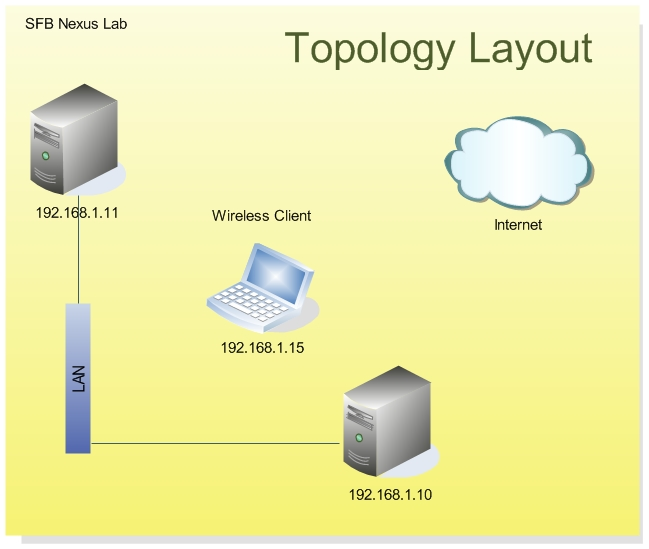
\includegraphics[width=0.8\textwidth]{images/Labor.jpg}
  \caption{Topologie}
  \label{fig:Topologie}
\end{figure}

\subsection{Software}

\subsubsection{Betriebssystem}

Auf den Rechnern mit der Wistron CM9 Atheros AR5213A WLAN-Karte wurde
als Betriebssystem Fedora 6 mit Linux Kernel 2.6.18
und auf dem Laptop Windows XP verwendet.

\subsubsection{Treiber f"ur WLAN-Karten}

In diesem Abschnitt wird beschrieben, wie man Treiber f"ur WLAN-Karten
auf den beiden Rechnern und Laptop installiert und die WLAN-Karten
konfiguriert werden k"onnen.

Auf den Rechnern mit der Wistron CM9 Atheros AR5213A WLAN-Karte
wurde die letzte Version des MadWifi-Treibers zuerst kompiliert und dann
installiert.

Kompilieren des MadWifi-Treibers:
\begin{shelllst}
svn checkout http://svn.madwifi.org/madwifi/trunk madwifi
cd madwifi
make
\end{shelllst}

Installieren des kompilierten MadWifi-Treibers (\textbf{root}-Rechte ben"otigt):
\begin{shelllst}
make install
\end{shelllst}

Manuelles Laden des MadWifi-Treibers (\textbf{root}-Rechte ben"otigt):
\begin{shelllst}
modprobe ath_pci
\end{shelllst}

Automastische Laden des MadWifi-Treibers beim Booten
(\textbf{root}-Rechte ben"otigt):
\begin{shelllst}
mkdir /etc/modules.autoload.d/
echo ath_pci >> /etc/modules.autoload.d/kernel-2.6
\end{shelllst}

Nachdem der MadWifi-Treiber geladen wurde (manuell oder automatisch),
kann die WLAN-Karte konfiguriert werden. Die WLAN-Karte kann entweder
manuell oder automatisch beim Booten konfiguriert werden.

Manuelles Konfigurieren der WLAN-Karte (\textbf{root}-Rechte ben"otigt):
\begin{shelllst}
ifconfig ath1 inet 192.168.2.1/24 # IP-Adresse
iwconfig ath1 essid mesh          # SSID="mesh"
iwconfig ath1 mode ad-hoc         # Ad-Hoc Modus einschalten
iwconfig ath1 channel 36          # 802.11a Kanal 36
iwconfig ath1 enc s:1234567890abc # 108 bit WEP-Passwort
                                  # (13 Zeichen)
\end{shelllst}

Damit die WLAN-Karte beim Booten von Fedora 6
automatisch konfiguriert werden kann, muss eine Konfigurationsdatei
mit dem Namen \textbf{ifcfg-ath1} im Verzeichnis
\textbf{/etc/sysconfig/network-scripts} angelegt werden.

Listing der Datei \textbf{/etc/sysconfig/network-scripts/ifcfg-ath1}:
\begin{shelllst}
cat /etc/sysconfig/network-scripts/ifcfg-ath1
DEVICE=ath1
ONBOOT=yes
			
BOOTPROTO=static
IPADDR=192.168.2.1
NETMASK=255.255.255.0
			
ESSID=mesh
MODE=ad-hoc
CHANNEL=36
KEY=s:1234567890abc
\end{shelllst}

Nachdem die Datei \textbf{/etc/sysconfig/network-scripts/ifcfg-ath1}
erstellt wurde, muss Init-Skripot f"ur Netzwerk-Dienste neugestartet
werden (\textbf{root}-Rechte ben"otigt):
\begin{shelllst}
/etc/init.d/network restart
\end{shelllst}

Den offiziellen Windows-Treiber f"ur die Intel Wireless WiFi Link 4965AGN
WLAN-Karte kann auf der Intel-Webpage heruntergeladen werden. Die Anleitung
zur Installation und Konfiguration diesr WLAN-Karte findet man auch
auf der selben Webpage (siehe \ref{Intel Wireless WiFi Link 4965AGN}) und
wird hier nicht weiter beschrieben.

\subsubsection{olsrd}

In diesem Abschnitt wird erkl"art, wie man den olsr.org OLSR daemon kompiliert,
installiert und konfiguriert. Au"serdem wird hier auch gezeigt, wie man
Plugins f"ur den olsr.org OLSR daemon kompiliert uns installiert.

Kompilieren des OLSR daemons:
\begin{shelllst}
cvs -d:pserver:anonymous@olsrd.cvs.sourceforge.net:\
	/cvsroot/olsrd login
cvs -z3 -d:pserver:anonymous@olsrd.cvs.sourceforge.net:\
	/cvsroot/olsrd co olsrd-current
cd olsrd-current
make
\end{shelllst}

Installieren des OLSR daemons (\textbf{root}-Rechte ben"otigt):
\begin{shelllst}
make install
\end{shelllst}

Im Folgenden wird demonstriert, wie man
das HTTP Mini-Server Plugin \textbf{httpinfo} kompiliert und installiert.
Das Plugin \textbf{httpinfo} ist ein kleiner und einfacjer HTTP-Server und
erlaubt es, z.B. die Routing-Tabelle eines Knotens in einem Mesh-Netzwerk
zu erfassen.

Damit die Topology eines Mesh-Netzwerkes visualisiert werden kann,
muss noch das Dot Data Generation Plugin \textbf{dot\_draw}
kompiliert und installiert werden. Das Plugin \textbf{dot\_draw}
ist auch ein kleiner Server. Wenn man eine TCP-Verbindung zu diesem Server
aufbaut (z.B mit \textbf{netcat} oder \textbf{telnet}),
dann bekommt man die aktuelle Topology des Mesh-Netzwerkes in
Form eines Dot-Graphes
(siehe GrpahViz \url{http://www.graphviz.org} und
 \url{de.wikipedia.org/wiki/DOT\_(GraphViz)}).
Dieser Dot-Graph ist eine einfache Textdatei und kann mit Hilfe des
Programms \textbf{dot} zu einem Bild konvertiert werden.

Es gibt noch andere zahlreiche Plugins f"ur
den olsr.org OLSR daemon. Sie alle k"onnen auf dieselbe Weise kompiliert
und installiert werden.

Kompilieren des HTTP Mini-Server Plugins \textbf{httpinfo}:
\begin{shelllst}
cd lib/httpinfo
make
\end{shelllst}

Installieren des HTTP Mini-Server Plugins \textbf{httpinfo}
(\textbf{root}-Rechte ben"otigt):
\begin{shelllst}
make install 
chcon -t textrel_shlib_t /usr/lib/olsrd_httpinfo.so.0.1
\end{shelllst}

Der olsr.org OLSR daemon wird "uber die Datei \textbf{/etc/olsrd.conf}
konfiguriert.  Das vollst"andige Listing der Datei \textbf{/etc/olsrd.conf} ist
im Anhang angegeben (siehe \ref{olsrd.conf}).
Es muss vor allem das Netzwerk-Interface und Plugins konfiguriert werden.

Starten des olsr.org OLSR daemons
(\textbf{root}-Rechte ben"otigt):
\begin{shelllst}
olsrd
\end{shelllst}

Der olsr.org OLSR daemon kann auch automatisch beim Starten
des Betriebssystems gestartet werden. Daf"ur muss ein Startup-Skript
\textbf{/etc/init.d/olsrd} erzeugt werden. Das Listing der Datei
\textbf{/etc/init.d/olsrd} kann man hier betrachten \ref{olsrd_startup}.

Nachdem die Date erzeugt wurde, muss noch das System so konfiguriert
werden, das das Startup-Skript \textbf{/etc/init.d/olsrd} beim Booten
ausgef"uhrt werden kann (\textbf{root}-Rechte ben"otigt):
\begin{shelllst}
chmod 755 /etc/init.d/olsrd
chkconfig --add olsrd
\end{shelllst}

Das Kompilieren und Konfigurieren des olsr.org OLSR daemons f"ur Windows XP
wird hier nicht erkl"art, weil es ziehmlich kompliziert ist. Wir haben
den olsr.org OLSR daemon und die GUI zu ihm f"ur Windows XP selbst kompiliert
und konfiguriert. Um den olsr.org OLSR daemon zu kompilieren, wird cygwin
mit gcc ben"otigt. Um die GUI f"ur den olsr.org OLSR daemon zu kompilieren,
wird Microsoft Visual C++ 2005 ben"otigt.

\subsubsection{Visualisierung}

Das Dot Data Generation Plugin \textbf{dot\_draw} f"ur den olsr.org OLSR
daemon stellt die Topology eines Mesh-Netzwerkes in Form eines Dot-Graphes dar.
Der Dot-Graph ist eine Textdatei und man kann aus dieser Datei die Topology
nicht sofort sehen.

Um die aktuelle Topology mit einem Webbrowser online betrachten zu k"onnen,
haben wir auf einem Linux-Rechner in unserem Mesh-Netzwerk einen Apache
HTTP-Server installiert und ein CGI-Skript (Perl-Skript) entwickelt,
das die aktuelle Topology des Mesh-Netzwerkes grafisch darstellt.

Installieren des Pache HTTP-Servers in Fedora 6
(\textbf{root}-Rechte ben"otigt):
\begin{shelllst}
yup install httpd
\end{shelllst}

Das CGI-Skript, das die aktuelle Topology des Mesh-Netzwerkes vom
Dot Data Generation Plugin \textbf{dot\_draw} ausliest, ins Bild konvertiert
und in eine Webseite integriert, finden Sie hier \ref{topology.pl}.
Das CGI-Skript muss im Verzeichnis \textbf{/var/httpd/cgi-bin/} abgelegt
und ausf"uhrbar gemacht werden.

Das CGI-Skript \textbf{topology.pl} ben"otigt noch das Paket GraphViz,
konkret wird das Programm \textbf{dot} aus diesem Paket ben"otigt,
um Dot-Graphen zu Bildren konvertieren zu k"onnen.

Installieren des GraphViz-Pakets (\textbf{root}-Rechte ben"otigt):
\begin{shelllst}
yup install graphviz
\end{shelllst}

\subsubsection{dhcpd}

In unserem Test haben wir jedem Knoten in unsrem kleinen Mesh-Netzwerk
IP-Adressen statisch vergeben. Mit 3 Knoten im Netzwerk ist der Aufwand daf"ur
sehr gering. Wenn sich aber Knoten zum Mesh-Netzwerk dynamisch verbinden
und verschwinden k"onnen oder wenn die Anzahl der Knoten im Mesh-Netzwerk
sehr gro"s wird, dann kann man auf einem der Linux-Rechnern in unserem
Mesh-Netzwerk einen DHCP-Server installieren. Dieser Knoten
mit DHCP-Server muss nat"urlich st"andig im Mesh-Netzwerk vorhanden sein.

Installieren des DHCP-Servers in Fedora 6 (\textbf{root}-Rechte ben"otigt):
\begin{shelllst}
yup install dhcp
\end{shelllst}

Der DHCP-Server kann "uber die Datei \textbf{/etc/dhcpd.conf} konfiguriert
werden.

Damit der DHCP-Server automatisch beim Booten gestartet werden kann,
muss man folgendes Kommando ausf"uhren (\textbf{root}-Rechte ben"otigt):
\begin{shelllst}
chkconfig dhcpd on
\end{shelllst}

Manuelles Beziehen einer IP-Adresse vom DHCP-Server
(\textbf{root}-Rechte ben"otigt):
\begin{shelllst}
dhclient ath1
\end{shelllst}

\subsubsection{Firewall}

Damit der olsr.org OLSR daemon "uberhaupt korrekt funktionieren kann,
m"ussen mehrere Ports in der Firewall von beiden Rechnern ge"offnet werden.

Damit der OLSR-Protokoll funktionieren kann, muss der UDP-Port 698
f"ur eingehende Pakete ge"offnet werden (\textbf{root}-Rechte ben"otigt):
\begin{shelllst}
iptables -A RH-Firewall-1-INPUT -i ath1 -p udp\
	--sport 698 -j ACCEPT
\end{shelllst}

Damit man auf den HTTP Mini-Server \textbf{httpinfo} eines Knotens zugreifen
kann, muss der TCP-Port
(hier 8080, kann in der \textbf{/etc/olsrd.conf} konfiguriert werden)
des Servers f"ur eingehende Pakete ge"offnet werden
(\textbf{root}-Rechte ben"otigt):
\begin{shelllst}
iptables -A RH-Firewall-1-INPUT -p tcp --dport 8080\
	-m state --state NEW -j ACCEPT
\end{shelllst}

Damit man auf den Dot Data Generation Server \textbf{dot\_draw}
eines Knotens zugreifen kann, muss der TCP-Port
(hier 8081, kann in der \textbf{/etc/olsrd.conf} konfiguriert werden)
des Servers f"ur eingehende Pakete ge"offnet werden
(\textbf{root}-Rechte ben"otigt):
\begin{shelllst}
iptables -A RH-Firewall-1-INPUT -p tcp --dport 8081\
	-m state --state NEW -j ACCEPT
\end{shelllst}

Um die aktuelle Topology unseres Mesh-Netzwerkes betrachten zu k"onnen,
muss man den TCP-Port 80 f"ur eingehende Verbindungen "offnen
(\textbf{root}-Rechte ben"otigt):
\begin{shelllst}
iptables -A RH-Firewall-1-INPUT -p tcp --dport http\
	-m state --state NEW -j ACCEPT
\end{shelllst}

Wenn im Mesh-Netzwerk ein DHCP-Server verwendet werden soll, dann
m"ussen auf jedem Knoten im Mesh-Netzwerk die UDP-Ports 67 und 68
ge"offnet werden (\textbf{root}-Rechte ben"otigt):
\begin{shelllst}
-A RH-Firewall-1-INPUT -i ath1 -p udp\
	--sport 67:68 --dport 67:68 -j ACCEPT
\end{shelllst}

Damit alle diese Ports automatisch beim Starten des Betriebssystems
ge"offnet werden k"onnen, muss in Fedora 6
die Datei \textbf{/etc/sysconfig/iptables} erweitert werden
(\textbf{root}-Rechte ben"otigt):
\begin{shelllst}
cat >> /etc/sysconfig/iptables << EOF
-A RH-Firewall-1-INPUT -i ath1 -p udp\
	--sport 698 -j ACCEPT
-A RH-Firewall-1-INPUT -p tcp --dport 8080\
	-m state --state NEW -j ACCEPT
-A RH-Firewall-1-INPUT -p tcp --dport 8081\
	-m state --state NEW -j ACCEPT
-A RH-Firewall-1-INPUT -p tcp --dport http\
	-m state --state NEW -j ACCEPT
EOF

/etc/init.d/iptables restart
\end{shelllst}

Die Konfiguration der Windows-Firewall auf dem Laptop wird hier nicht erkl"art,
siehe entsprechende Literatur und Artikel im Internet.

\subsection{Inbetriebnahme}

Nachdem alle Treiber, der OLSR daemon und Plagins kompiliert und installiert
wurden und entsprechende Ports in Firewall ge"offnet wurden,
kann auf jedem Knoten der OLSR daemon gestartet werden.

\subsection{Ergebnisse}

In diesem Abschnitt werden wir die Ergebnisse von unserem Test pr"asentieren.

\subsubsection{Topologie}

Auf dem Bild \ref{fig:Topology} kann man die Topologie des Mesh-Metzwerkes
betrachten. Der Knoten mit der IP-Adresse 192.168.2.15 ist der Laptop und
die anderen beiden sind Linux-Rechner. Der rechteckige Knonten auf dem Bild, ist
der Knoten, der diese Topologie erzeugt hat.

\begin{figure}[H]
\centering
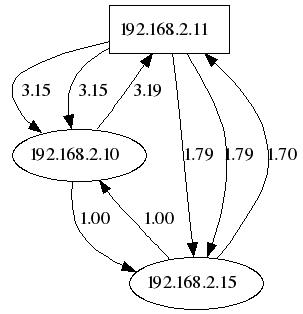
\includegraphics[width=0.5\textwidth]{images/Topology.jpg}
\caption{Topologie dargestellt mit dem olsr.org Plugin \textbf{dot\_draw}}
\label{fig:Topology}
\end{figure}

\subsubsection{Routing-Tabelle}

Auf dem Bild \ref{fig:httpinfo} kann man die Routing-Tabelle
eines Linux-Rechners betrachten

\begin{figure}[H]
\centering
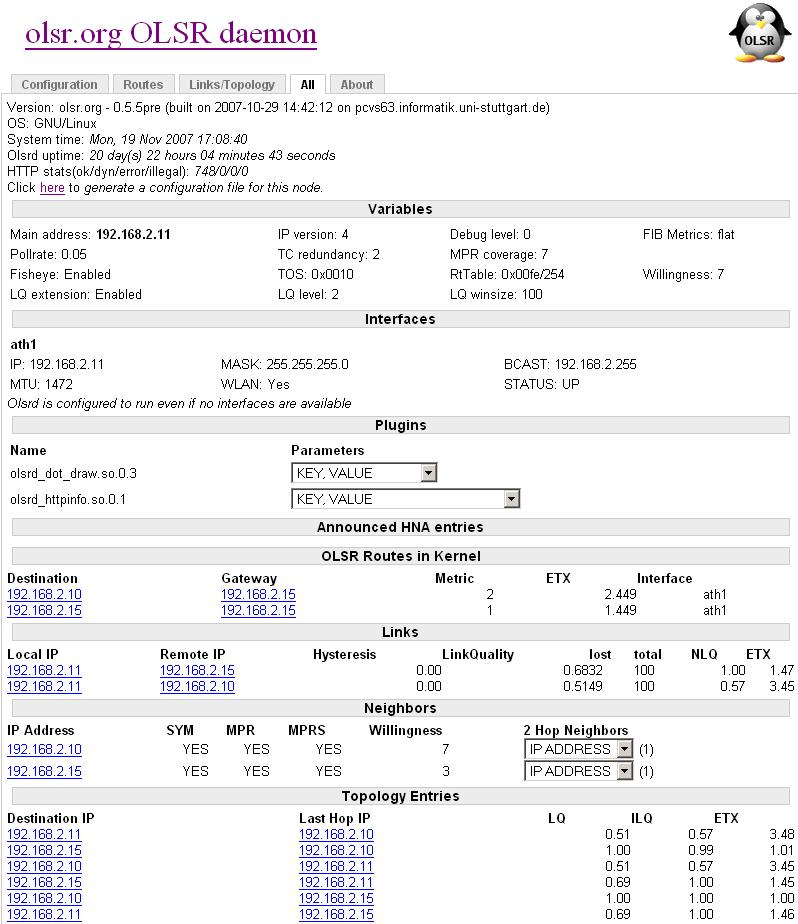
\includegraphics[width=1.0\textwidth]{images/Olsr_Route.jpg}
\caption{Routing-Tabelle eines Knotens dargestellt
	mit dem olsr.org Plugin \textbf{httpinfo}}
\label{fig:httpinfo}
\end{figure}

\section{Fazit}

\subsection{�bersicht}

Dieser Abschnitt stellt ein "Ubersicht "uber aktuelle verf"ugbare 
Hardwareplattformen und Systemsoftware f"ur WMN dar.
	
\begin{figure}[htbp]
\begin{center}
\setlength{\extrarowheight}{4pt}
\begin{tabular}{|l|c|c|c|c|c|c|c|c|c|c|}
\hline
% HEAD BEGIN
 &
\rotatebox{90}{IEEE 802.11a} & \rotatebox{90}{Ad-Hoc Modus} &
\rotatebox{90}{Treiber (Linux/Windows)} & \rotatebox{90}{Open-Source Firmware} &
\rotatebox{90}{LAN-Anschluss} & \rotatebox{90}{Sicherheit} &
\rotatebox{90}{Installation} & \rotatebox{90}{Konfiguration} &
\rotatebox{90}{Mini-PCI Slot} & \rotatebox{90}{IEEE 802.11n}\\
% HEAD END
\hline
Linksys WMP55AG                  & ++  & + & ++ & -   & ++ & ++  & + & + & -  & - \\
\hline
Netgear WAG311                   & ++  & + & ++ & -   & ++ & ++  & + & + & -  & - \\
\hline
D-Link DWL-A520                  & +   & + & ++ & -   & ++ & +   & + & + & -  & - \\
\hline
Gigabyte GN-WPEAG                & ++  & + & ++ & -   & ++ & +++ & + & + & -  & - \\
\hline
Intel PRO/Wireless 5000          & +   & + & +  & -   & ++ & +   & + & + & -  & - \\
\hline
D-Link DWL-AG530                 & ++  & + & ++ & -   & ++ & +++ & + & + & -  & - \\
\hline
D-Link DWL-G550                  & ++  & + & ++ & -   & ++ & +++ & + & + & -  & - \\
\hline
\hline
Wistron CM9 Atheros AR5213A      & ++  & + & ++ & -   & ++ & +++ & + & + & -  & - \\
\hline
Intel PRO/Wireless 3945          & ++  & + & ++ & -   & ++ & +++ & + & + & -  & - \\
\hline
Intel PRO/Wireless 2915          & ++  & + & ++ & -   & ++ & +++ & + & + & -  & - \\
\hline
Intel Wireless WiFi Link 4965AGN & +++ & + & ++ & -   & ++ & +++ & + & + & -  & + \\
\hline
\hline
Linksys WRT54G v1.0              & ++  & + & -  & ++  & +  & +++ & - & + & +  & - \\
\hline
Linksys WRT55AG                  & ++  & + & -  & +   & +  & +   & - & + & ++ & - \\
\hline
Asus WL500G/GP                   & ++  & + & -  & +++ & +  & +++ & - & + & +  & - \\
\hline
Netgear HR314                    & +   & - & -  & -   & +  & +   & - & + & -  & - \\
\hline
\end{tabular}
\end{center}
\caption{�bersicht und Bewertung von  Hardware}
\end{figure}

\begin{figure}[htbp]
\begin{center}
\setlength{\extrarowheight}{4pt}
\begin{tabular}{|l|c|c|c|c|}
\hline
% HEAD BEGIN
 &
\rotatebox{90}{Betriebssysteme} & \rotatebox{90}{Installation} &
\rotatebox{90}{Konfiguration} & \rotatebox{90}{Visualisierung}\\
% HEAD END
\hline
OLSRD        & +++ & + & + & ++ \\
\hline
B.A.T.M.A.N. & +   & + & + & -  \\
\hline
Meshcom & +   & + & - & +  \\
\hline
\end{tabular}
\end{center}
\caption{�bersicht und Bewertung von Software}
\end{figure}
	
\subsection{Empfehlung f"ur ein geeignetes WMN}

Um eines stabiles, f"ur die Forschung geeignets Mesh-Netzwerk aufzubauen, 
sind vor allem folgende Hardware zu empfehlen: 

\begin{itemize}
	\item PCs + Wlan Karten mit Atheros Chipsatz (z.b \emph{Wistron CM9 Atheros AR5213A})
\end{itemize}

Weiterhin kann das Mesh-Netzwerk zu einem heterogenen WMN erweitert werden, 
indem folgende WLAN-Router eingesetzt werden:

\begin{itemize}
	\item Linksys WRT54G v1.0  
\end{itemize}

Als Software-System f"ur das aufzubauende WMN hat sich \emph{olsrd}
als besonders geeignet erwiesen. 

Um die gesamte Informatikgeb"aude abzudecken, w"urden ca. 30-44 PCs reichen.
Das heist ca. 10-15 PCs pro Stock.
%(TODO) BILD!
%Jeder Rechner ist dabei mit zwei Wlan-Karten zu gestaten, um MIMO zu realisieren..
Kosten f"ur die notwendige Hardware liegen damit unter der Budget-Grenze.
%(TODO)

%---------------------------------------------------------------------&

\section{Anhang}

\subsection{olsrd.conf}
\label{olsrd.conf}

Listing der Datei \textbf{/etc/olsrd.conf}:
\lstinputlisting[language=bash,backgroundcolor=\color{shelllstbgcolor}]
{olsrd.conf}

\subsection{olsrd Startup-Skript}
\label{olsrd_startup}

Listing der Datei \textbf{/etc/init.d/olsrd}:
\lstinputlisting[language=bash,backgroundcolor=\color{shelllstbgcolor}]
{olsrd_startup}

\subsection{topology.pl}
\label{topology.pl}

Listing der Datei \textbf{/var/htppd/cgi-bin/topology.pl}:
\lstinputlisting[language=Perl,backgroundcolor=\color{shelllstbgcolor}]
{topology.pl}


%---------------------------------------------------------------------&
\end{document}
